\documentclass{article}
\usepackage{epsfig, latexsym}

\begin{document}

\newcommand{\SOPmin}{${\rm SOP}_{\rm min} \ $}
\newcommand{\POSmin}{${\rm POS}_{\rm min} \ $}
\newcommand{\bs}{\backslash}
\newcommand{\x}{\addtocounter{enumi}{1} \theenumi}


\title{
\Huge{CSE 271}\\
\normalsize{Exam 3}\\
\normalsize{Return this document!!!}\\
\makebox[4in][l]{Name:}
SSN:}
\date{}

\maketitle{}

\begin{enumerate}
\item {\bf (3 pts.)} How many \SOPmin realizations does F have?
F(A,B,C,D)=$\Sigma$m(0,1,2,5,6,8,11,12,15)

$$ \begin{array} {c||c|c|c|c}
        AB \bs CD & 00 & 01 & 11 & 10 \\ \hline \hline
        00        &    &    &    &    \\ \hline
        01        &    &    &    &    \\ \hline
        11        &    &    &    &    \\ \hline
        10        &    &    &    &    \\
\end{array} $$ 

\begin{tabular}{p{0.75in}p{0.75in}p{0.75in}p{0.75in}p{0.75in}}
a) 1 & b) 2 & c) 3 & d) 4 & e) 5 \\
\end{tabular}

\item {\bf (3 pts.)} The output of a sequential circuit is fundamentally
different than a combinational circuit because its output is a function
of the?
\begin{description}
\item{a) } State
\item{b) } Input
\item{c) } Output
\item{d) } Number of inputs
\item{e) } The staple monkey
\end{description}

\item {\bf (2 pts.)} You are told to implement a 3 bit counter using our seven
step FSM design process.  Each state represents the current count value.  The
state assignment is performed using a dense encoding. 
How many flip flops will this FSM require?

\begin{tabular}{p{0.75in}p{0.75in}p{0.75in}p{0.75in}p{0.75in}}
a) 3 & b) 4 & c) 7 & d) 8 & e) 16 \\
\end{tabular}

\item {\bf (2 pts.)} You are told to implement a 3 bit counter using the
ones hot design process.  Each state represents the current count value. 
How many flip flops will the counter require?

\begin{tabular}{p{0.75in}p{0.75in}p{0.75in}p{0.75in}p{0.75in}}
a) 3 & b) 4 & c) 7 & d) 8 & e) 16 \\
\end{tabular}

\pagebreak
Questions 5-8 concern the FSM realization of the state diagram given below.
Assume a ones hot encoding of the states.  Call the input $X$ and the output 
$Z$.  Let $D_A$ be the input to the flip flop representing state $A$.  Let $Q_A$ 
be the output from the flip flop representing state $A$.  Apply the preceding 
definitions to $D_B, Q_B, D_C, Q_C$.

\item {\bf (1 pts.)} How many flip flops are required to realize this FSM?

\begin{tabular}{p{0.75in}p{0.75in}p{0.75in}p{0.75in}p{0.75in}}
a) 1 & b) 2 & c) 3 & d) 4 & e) 4 \\
\end{tabular}

\item {\bf (3 pts.)} What is the memory input equation for flip flop $A$?
\begin{description}
\item{a) } 1
\item{b) } 0
\item{c) } $X'Q_A$
\item{d) } $XD_C$
\item{e) } None of the above.
\end{description}

\item {\bf (3 pts.)} What is the memory input equation for flip flop $R$?
\begin{description}
\item{a) } 1
\item{b) } 0
\item{c) } $X'Q_A$
\item{d) } $XD_C$
\item{e) } None of the above.
\end{description}
\includegraphics[-60mm,15mm][0mm,15.1mm]{./Fig3/sd.eps}
\item {\bf (3 pts.)} What is the equation for $Z$?
\begin{description}
\item{a) } $X'Q_A + X'Q_B + X'Q_C$
\item{b) } $X'+Q_C$
\item{c) } $X'D_C + X'D_B + X'D_A$
\item{d) } $X' + D_C$
\item{e) } None of the above.
\end{description}

\pagebreak
Given the following state diagram and state assignment answer 
questions 9-12.  The input to the FSM is called $x$.

\begin{tabular}{l||ll}
State & $Q_1$ & $Q_0$ \\ \hline \hline
R	& 0 & 0 \\ \hline
A	& 0 & 1 \\ \hline
B	& 1 & 0 \\ \hline
C	& 1 & 1 \\ 
\end{tabular}

\includegraphics[-70mm,25mm][0mm,25.1mm]{./Fig3/sd.eps}

\item {\bf (3 pts.)} What is the output equation for $Z$?
\begin{description}
\item{a) } $Q_1 + Q_0$
\item{b) } $Q_1'Q_0 + Q_1Q_0'$
\item{c) } $xQ1' + x'Q1 + Q_1Q_0'$
\item{d) } $x + Q_1Q_0'+Q_1Q_0$
\item{e) } None of the above.
\end{description}

\item {\bf (3 pts.)} What is the memory input equation for $D_1$?
\begin{description}
\item{a) } $Q_1 + Q_0$
\item{b) } $Q_1'Q_0 + Q_1Q_0'$
\item{c) } $xQ1' + x'Q1 + Q_1Q_0'$
\item{d) } $x + Q_1Q_0'+Q_1Q_0$
\item{e) } None of the above.
\end{description}

\item {\bf (3 pts.)} What is the memory input equation for $D_0$?
\begin{description}
\item{a) } $Q_1 + Q_0$
\item{b) } $Q_1'Q_0 + Q_1Q_0'$
\item{c) } $xQ1' + x'Q1 + Q_1Q_0'$
\item{d) } $x + Q_1Q_0'+Q_1Q_0$
\item{e) } None of the above.
\end{description}

\item {\bf (3 pts.)} If $(Q_1, Q_0)= (0,1)$ and a clock edge arrives
then what will the output become after the clock edge?

\begin{tabular}{p{0.5in}p{0.5in}p{3.00in}}
a) 1 & b) 0 & c) Cannot answer question with given information.  \\
\end{tabular}

\pagebreak
For questions 13-16 assume that you have constructed a circuit
which is involved in a 2-line handshake; your circuit
is a passive consumer of data.  

\item {\bf (3 pts.)} Which of the following explanations justifies 
waiting for the request to be lowered before processing the data?
\begin{description}
\item{a) } The external world may be much faster than your circuit.
\item{b) } The external world may be much slower than your circuit.
\item{c) } The external world may be the same speed as your circuit.
\item{d) } The external world may be busy.
\item{e) } Our circuit may be busy.
\end{description}

\item {\bf (3 pts.)} Which of the following explanations justifies asserting
an acknowledgement after you latch the data?
\begin{description}
\item{a) } The external world may be much faster than your circuit.
\item{b) } The external world may be much slower than your circuit.
\item{c) } The external world may be the same speed as your circuit.
\item{d) } The external world may be busy.
\item{e) } Our circuit may be busy.
\end{description}

\item {\bf (3 pts.)} What role does the external world play in the 
2-line handshake?
\begin{description}
\item{a) } Active producer
\item{b) } Passive producer
\item{c) } Active consumer
\item{d) } Passive consumer
\end{description}

\item {\bf (3 pts.)} Who generates the REQ signal?
\begin{description}

\begin{tabular}{p{1.75in}p{1.75in}}
a) The external world & b) Our Circuit \\
\end{tabular}
\end{description}

\pagebreak
For questions 17-19 use the algorithm and the corresponding piece 
of the control unit below.

\includegraphics[-60mm,50mm][0mm,51mm]{./Fig3/branch.eps}

\begin{verbatim}
if (x=1) then 
    if (y=1) then A=A+1;
    else          B=B+1;
else        
    if (y=1)      C=C+1;
    else          D=D+1;
\end{verbatim}
\vspace{16mm}


\item {\bf (3 pts.)} In which state does D get incremented?

\begin{tabular}{p{0.75in}p{0.75in}p{0.75in}p{0.75in}p{0.75in}}
a) S4 & b) S5 & c) S6 & d) S7 & e) other \\
\end{tabular}

\item {\bf (3 pts.)}Assume that X=1 and Y=1.  Given the partial timing 
diagram below, about what time will the outputs of the A register 
equal A+1?

\begin{tabular}{p{0.75in}p{0.75in}p{0.75in}p{0.75in}p{0.75in}}
a) 40nS & b) 60nS & c) 80nS & d) 120nS & e) 140nS \\
\end{tabular}

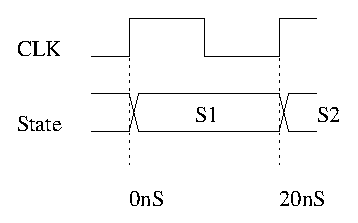
\includegraphics{./Fig3/time.eps}

\item {\bf (3 pts.)} How many states can the control unit be
reduced to, assuming that you keep state S1?

\begin{tabular}{p{0.75in}p{0.75in}p{0.75in}p{0.75in}p{0.75in}}
a) 1 & b) 4 & c) 5 & d) 6 & e) 7 \\
\end{tabular}

\pagebreak
Questions 20-44 {\bf (1 pt. each)}, questions 45-48 deal with the construction 
of a digital circuit to accomplish the task specified by the following 
algorithm.  A(0) refers to the LSB of A.  A$>>$ 1 refers to A shifted right 
1 bit.

{\small
\begin{verbatim}
while(1) {
    while(REQ == 0);              // If the control bit equals 0 or 00  mark A 
    A = datainA;                  // If the control bit equals 01       mark B 
    B = datainB;                  // If the control bit equals 10       mark C 
    ACK = 1;                      // If the control bit equals 1 or 11  mark D 
    while (REQ == 1);             // If the control bit is a don't care mark E 
    ACK = 0;
    C = 0;
    for (i=0; i<B; i++) {
        if (A(0) == 1) then
            C = C + 1;
        else 
            C = C - 1;
        A = A >> 1;
}   } 
\end{verbatim}}
\begin{figure}[ht]
\centerline{\psfig{figure=./Fig3/dp&cu.eps,width=5in.,clip=}}
\end{figure}

\begin{tabular}{|l||l|l|l|l|l|l|l|}  \hline
State & ACK & A       & B      & C      & Mux        & count   & Add/Sub \\ \hline
      & 0   & 00 hold & 0 hold & 0 hold & 0 pass 0   & 00 hold & 0 add \\ \hline
      & 1   & 01 SR   & 1 load & 1 load & 1 pass C$\pm$1 & 01 down & 1 sub \\ \hline
      &     & 10 SL   &        &        &            & 10 up   &       \\ \hline
      &     & 11 load &        &        &            & 11 load &       \\ \hline   \hline
Wait1 & \x  &         &        &        &            &         &       \\ \hline
Get   & \x  &  \x     &  \x    &  \x    &  \x        &  \x     & \x    \\ \hline
Wait2 & \x  &  \x     &        &        &  \x        &  \x     &       \\ \hline
For/If &    &         &        &        &            &         &       \\ \hline
Inc   &     &  \x     &        &  \x    &  \x        &         & \x    \\ \hline
Dec   & \x  &         &        &  \x    &  \x        &         & \x    \\ \hline
Shift &     &  \x     &  \x    &  \x    &  \x        &         & \x    \\ \hline
\end{tabular}

\pagebreak
\item{\bf (3 pts.)} How many bits are in the status word (inputs to the 
control unit)?

\begin{tabular}{p{0.75in}p{0.75in}p{0.75in}p{0.75in}p{0.75in}}
a) 1 & b) 2 & c) 4 & d) 5 & e) 9 \\
\end{tabular}

\item{\bf (3 pts.)} How many bits are in the control word (outputs from the 
control unit)?

\begin{tabular}{p{0.75in}p{0.75in}p{0.75in}p{0.75in}p{0.75in}}
a) 1 & b) 2 & c) 4 & d) 5 & e) 9 \\
\end{tabular}

\item {\bf (3 pts.)} Let A be N bits wide.  Let B's range be $[0,log_2(N)]$.
How many bits wide is the B register?

\begin{tabular}{p{1.30in}p{1.30in}p{2.00in}}
a) $log_2(log_2(N))$ & b) $log_2(log_2(N))+1$ &   \\
c) $log_2(N)$ & d) $log_2(N)+1$ & e) None of these.\\
\end{tabular}

\item {\bf (3 pts.)} Use the same assumptions about A and B as stated in the previous
problem.  How many bits wide does the C register need to be?

\begin{tabular}{p{1.30in}p{1.3in}p{2.00in}}
a) $log_2(log_2(N))+1$ & b) $log_2(N)+1$ &   \\
c) $N+1$ & d) $2^N+1$ & e) None of these.\\
\end{tabular}
\vspace{5mm}

Questions 49-50 deal with the following figure.  Assume that the
setup, hold, and propagation delay of the flip flops is 2 nS.

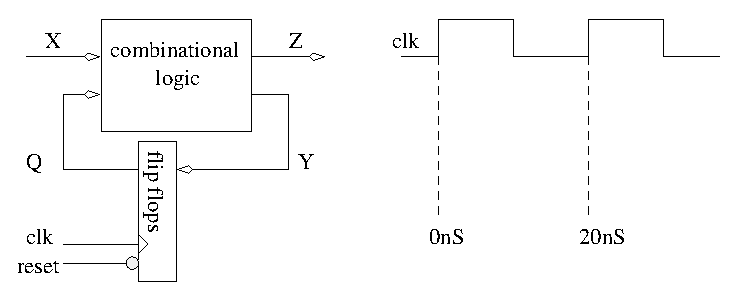
\includegraphics{./Fig3/fsm.eps}

\item {\bf (3 pts.)}Under what conditions will the flip flops be reset.
\begin{description}
\item{a) } When the clock rises and reset = 1.
\item{b) } When reset = 1.
\item{c) } When the clock rises and reset = 0.
\item{d) } When reset = 0.
\item{e) } None of the above.
\end{description}

\item {\bf (3 pts.)}At which of the following times does Q change?

\begin{tabular}{p{0.75in}p{0.75in}p{0.75in}p{0.75in}p{0.75in}}
a) 20nS  & b) 22nS  & c) 24nS & d) 26nS & e) 28nS \\
\end{tabular}

\pagebreak
\item {\bf (16 pts.)} A 8kx32 RAM is full of integer data.  You are to 
design a circuit that determines the sum of the integers between
addresses $A$ and $B$, inclusive.  You may assume that $A<B$ and that the 
values of $A$ and $B$ are already stored in registers.  The sum 
is to be placed in a 32 bit register called $S$.  Show:

\begin{tabular}{p{1.50in}p{0.25in}}
Datapath	& 6pts. \\
Control		& 6pts. \\
Control Word	& 1pt. \\
Binary Microinstruction & 3pts \\
\end{tabular}

\pagebreak
%% This is an ABET survey
%% Edited 12/2005 to include program outcomes
%% Edited 12/2008 to remove program outcomes

%% \begin{center} 
%% CSE 271 -- Introduction to Digital Systems \\
%% Course Objectives Survey \\ 
%% Penn State Erie, The Behrend College
%% \end{center}

\small{
In order to assure the continued success of the Behrend ECE
program, I would appreciate your evaluation of whether or
not this course met its learning objectives.  All answers
will be kept anonymous and will be used for the future 
improvement of this course and the entire ECE program.
Please record your answers on the SCANTRON form.
Thanks for your help.
}

\begin{tabular}{p{0.25in}p{2.5in}|p{0.45in}|p{0.4in}|p{0.4in}|p{0.4in}|p{0.4in}|} \\ \cline{3-7}
    &  & 
{\scriptsize Strongly Disagree} A & 
{\scriptsize Disagree} B & 
{\scriptsize Neutral} C & 
{\scriptsize Agree} D & 
{\scriptsize Strongly Agree} E \\ \hline

\item & I understand how to convert numbers from one base to another and 
how to add and subtract numbers represented in binary and 2's complement 
form. 
 & & & & & \\ \hline

\item & I understand how to convert between a truth table, a circuit diagram,
boolean expression and a word statement.
 & & & & & \\ \hline

\item & I understand how to simplify logic expression into SOP or
POS minimal form with or without don't cares.
 & & & & & \\ \hline

\item & I understand how to use ESPRESSO to minimize combinational logic
functions.
 & & & & & \\ \hline

\item & I understand how adders, comparators, multiplexers and decoders 
are built and how they operate. 
 & & & & & \\ \hline

\item & I understand how D,T,SR,JK, latches, clock latches and flip flops 
are supposed to operate. 
 & & & & & \\ \hline

\item & I understand how registers, shift registers, counters, tri-state 
logic and RAMs are built and how they should operate. 
 & & & & & \\ \hline

\item & I understand how to design Finite State Machines using a dense 
or Ones Hot encoding. 
 & & & & & \\ \hline

\item & I understand how to implement complex digital systems using the 
datapath and control design approach. 
 & & & & & \\ \hline

\end{tabular}


\end{enumerate}

\end{document}
